\subsection{Fórmulas explícitas para los primeros vectores (máximo hasta el cuarto) de la base $\cali{L}^{n}$}

Sea $n \in \IN$. Sea $0 \leq m \leq n-1$.
\TODO{revisa que estén bien !!1}
\[
\cali{L}^{n,0}_{m}=\frac{1}{\sqrt{n}}.
\]

Si $n \geq 2$,
\[
\cali{L}^{n,1}_{m}=\sqrt{\frac{3(n-1)}{n(n+1)}} \left( \frac{2}{n-1}m -1. \right)
\]

Si $n \geq 3$,
\[
\cali{L}^{n,2}_{m}=\sqrt{\frac{5(n-1)(n-2)}{n(n+1)(n+2)}} \left(1- \frac{6}{n-1}m + \frac{6}{(n-1)(n-2)}m(m-1) \right).
\]

Si $n \geq 4$,
\[
\cali{L}^{n,3}_{m}=-\sqrt{\frac{7(n-1)(n-2)(n-3)}{(n+3)(n+2)(n+1)n}}
\left( 1- \frac{12}{n-1}m + \frac{30}{(n-1)(n-2)}m(m-1)-
\frac{20}{(n-1)(n-2)(n-3)}m(m-1)(m-2) \right).
\]

\vspace{2cm}

Expresiones simplificadas (factorizadas) para $k=1,2$:

\[
\cali{L}^{n,1}_{m}=\frac{2\sqrt{3}}{(n+1)n(n-1)} \left( m-\frac{n-1}{2} \right)
\]

\[
\cali{L}^{n,2}_{m}=\frac{6\sqrt{5}}{\sqrt{(n+2)(n+1)n(n-1)(n-2)}} \left(
\left( m-\frac{n-1}{2} \right)^{2}+\frac{n-1}{4}(23n-47)
\right)
\]




\subsection{Fórmulas explícitas de la base $\cali{L}^{n}$ para dimensiones $2 \leq n \leq 6$} \label{subsect:Formulas explicitas}
\label{formulas explicitas para Ln con n de 2 hasta 6}

A continuación tabulamos los
elementos de la base de Legendre
discreta $\cali{L}^{n}$ para dimensiones
$2 \leq n \leq 6$.

%Tabla para n=2,3,4
\begin{center}
\begin{tabular}{ c c c c c c }
k $\backslash$ n & 2 & 3 & 4   \\ 
\hline

0 & $\left(
\frac{1}{\sqrt{2}}, \frac{1}{\sqrt{2}}\right)$ & 
$\left(\frac{1}{\sqrt{3}}, \frac{1}{\sqrt{3}}, \frac{1}{\sqrt{3}} \right)$ & 
$\left(\frac{1}{2}, \frac{1}{2}, \frac{1}{2}, \frac{1}{2} \right)$ \\ 
1 & $\left(-\frac{1}{\sqrt{2}}, \frac{1}{\sqrt{2}}\right)$ & 
$\left(-\frac{1}{\sqrt{2}}, 0, \frac{1}{\sqrt{2}} \right) $ & 
$\left(-\frac{3}{2\sqrt{5}}, -\frac{1}{2\sqrt{5}}, \frac{1}{2\sqrt{5}}, \frac{3}{2\sqrt{5}} \right)$  \\ 
2 & $---$ & $\left(\frac{1}{\sqrt{6}}, -\sqrt{\frac{2}{3}}, \frac{1}{\sqrt{6}} \right) $ & 
$\left(\frac{1}{2}, -\frac{1}{2}, -\frac{1}{2}, \frac{1}{2} \right)$ \\ 
3 & $---$ & $---$ & 
$\left(-\frac{1}{2\sqrt{5}}, \frac{3}{2\sqrt{5}}, -\frac{3}{2\sqrt{5}}, \frac{1}{2\sqrt{5}} \right)$  \\ 
\end{tabular}
\end{center} 
 
%Tabla para n=5,6
\begin{center}
\begin{tabular}{ c c c c c c }
k $\backslash$ n & 5 & 6  \\ 
\hline
0 & 
$\left(\frac{1}{\sqrt{5}}, \frac{1}{\sqrt{5}}, \frac{1}{\sqrt{5}},
\frac{1}{\sqrt{5}}, \frac{1}{\sqrt{5}} \right)$ 
& $\left(\frac{1}{\sqrt{6}}, \frac{1}{\sqrt{6}}, \frac{1}{\sqrt{6}},
\frac{1}{\sqrt{6}}, \frac{1}{\sqrt{6}}, \frac{1}{\sqrt{6}} \right)$ \\ 
1 &  
$\left(-\sqrt{\frac{2}{5}}, -\frac{1}{\sqrt{10}}, 0,
\frac{1}{\sqrt{10}}, \sqrt{\frac{2}{5}} \right)$  & 
$\left(-\sqrt{\frac{5}{14}}, -\frac{3}{\sqrt{70}}, -\frac{1}{\sqrt{70}},
\frac{1}{\sqrt{70}}, \frac{3}{\sqrt{70}}, \sqrt{\frac{5}{14}} \right)$ \\ 
2 & 
$\left(\sqrt{\frac{2}{7}}, -\frac{1}{\sqrt{14}}, -\sqrt{\frac{2}{7}},
-\frac{1}{\sqrt{14}}, \sqrt{\frac{2}{7}} \right)$ 
& $\left(\frac{5}{2\sqrt{21}}, -\frac{1}{2\sqrt{21}}, -\frac{2}{\sqrt{21}},
-\frac{2}{\sqrt{21}}, -\frac{1}{2\sqrt{21}}, \frac{5}{2\sqrt{21}} \right)$ \\ 
3 & 
$\left(-\frac{1}{\sqrt{10}}, \sqrt{\frac{2}{5}}, 0,
-\sqrt{\frac{2}{5}}, \frac{1}{\sqrt{10}} \right)$ &
$\left(-\frac{\sqrt{5}}{6}, \frac{7}{6\sqrt{5}}, \frac{2}{3\sqrt{5}},
-\frac{2}{3\sqrt{5}}, -\frac{7}{6\sqrt{5}}, \frac{\sqrt{5}}{6} \right)$ \\ 
4 & $\left(\frac{1}{\sqrt{70}}, -\frac{2\sqrt{2}}{\sqrt{35}}, 
\frac{3\sqrt{2}}{\sqrt{35}},
-\frac{2\sqrt{2}}{\sqrt{35}}, \frac{1}{\sqrt{70}} \right) $ & 
$\left(\frac{1}{2\sqrt{7}}, -\frac{3}{2\sqrt{7}}, \frac{1}{\sqrt{7}},
\frac{1}{\sqrt{7}}, -\frac{3}{2\sqrt{7}}, \frac{1}{2\sqrt{7}} \right)$ \\ 
5 & $---$ & 
$\left(-\frac{1}{6\sqrt{7}}, \frac{5}{6\sqrt{7}}, -\frac{5}{3\sqrt{7}},
\frac{5}{3\sqrt{7}}, -\frac{5}{6\sqrt{7}}, \frac{1}{6\sqrt{7}} \right)$ 
\end{tabular}
\end{center}


\begin{comment}

\begin{landscape}
\begin{center}
\begin{tabular}{ c c c c c c }
k $\backslash$ n & 2 & 3 & 4 & 5 & 6  \\ 
\hline

0 & $\left(\frac{1}{\sqrt{2}}, \frac{1}{\sqrt{2}}\right)$ & 
$\left(\frac{1}{\sqrt{3}}, \frac{1}{\sqrt{3}}, \frac{1}{\sqrt{3}} \right)$ & 
$\left(\frac{1}{2}, \frac{1}{2}, \frac{1}{2}, \frac{1}{2} \right)$ &
$\left(\frac{1}{\sqrt{5}}, \frac{1}{\sqrt{5}}, \frac{1}{\sqrt{5}},
\frac{1}{\sqrt{5}}, \frac{1}{\sqrt{5}} \right)$ 
& $\left(\frac{1}{\sqrt{6}}, \frac{1}{\sqrt{6}}, \frac{1}{\sqrt{6}},
\frac{1}{\sqrt{6}}, \frac{1}{\sqrt{6}}, \frac{1}{\sqrt{6}} \right)$ \\ 
1 & $\left(-\frac{1}{\sqrt{2}}, \frac{1}{\sqrt{2}}\right)$ & 
$\left(-\frac{1}{\sqrt{2}}, 0, \frac{1}{\sqrt{2}} \right) $ & 
$\left(-\frac{3}{2\sqrt{5}}, -\frac{1}{2\sqrt{5}}, \frac{1}{2\sqrt{5}}, \frac{3}{2\sqrt{5}} \right)$ &
$\left(-\sqrt{\frac{2}{5}}, -\frac{1}{\sqrt{10}}, 0,
\frac{1}{\sqrt{10}}, \sqrt{\frac{2}{5}} \right)$  & 
$\left(-\sqrt{\frac{5}{14}}, -\frac{3}{\sqrt{70}}, -\frac{1}{\sqrt{70}},
\frac{1}{\sqrt{70}}, \frac{3}{\sqrt{70}}, \sqrt{\frac{5}{14}} \right)$ \\ 
2 & $---$ & $\left(\frac{1}{\sqrt{6}}, -\sqrt{\frac{2}{3}}, \frac{1}{\sqrt{6}} \right) $ & 
$\left(\frac{1}{2}, -\frac{1}{2}, -\frac{1}{2}, \frac{1}{2} \right)$ &
$\left(\sqrt{\frac{2}{7}}, -\frac{1}{\sqrt{14}}, -\sqrt{\frac{2}{7}},
-\frac{1}{\sqrt{14}}, \sqrt{\frac{2}{7}} \right)$ 
& $\left(\frac{5}{2\sqrt{21}}, -\frac{1}{2\sqrt{21}}, -\frac{2}{\sqrt{21}},
-\frac{2}{\sqrt{21}}, -\frac{1}{2\sqrt{21}}, \frac{5}{2\sqrt{21}} \right)$ \\ 
3 & $---$ & $---$ & 
$\left(-\frac{1}{2\sqrt{5}}, \frac{3}{2\sqrt{5}}, -\frac{3}{2\sqrt{5}}, \frac{1}{2\sqrt{5}} \right)$ &
$\left(-\frac{1}{\sqrt{10}}, \sqrt{\frac{2}{5}}, 0,
-\sqrt{\frac{2}{5}}, \frac{1}{\sqrt{10}} \right)$ &
$\left(-\frac{\sqrt{5}}{6}, \frac{7}{6\sqrt{5}}, \frac{2}{3\sqrt{5}},
-\frac{2}{3\sqrt{5}}, -\frac{7}{6\sqrt{5}}, \frac{\sqrt{5}}{6} \right)$ \\ 
4 & $---$ & $---$ & 
$---$ & $\left(\frac{1}{\sqrt{70}}, -\frac{2\sqrt{2}}{\sqrt{35}}, 
\frac{3\sqrt{2}}{\sqrt{35}},
-\frac{2\sqrt{2}}{\sqrt{35}}, \frac{1}{\sqrt{70}} \right) $ & 
$\left(\frac{1}{2\sqrt{7}}, -\frac{3}{2\sqrt{7}}, \frac{1}{\sqrt{7}},
\frac{1}{\sqrt{7}}, -\frac{3}{2\sqrt{7}}, \frac{1}{2\sqrt{7}} \right)$ \\ 
5 & $---$ & $---$ & 
$---$ & $---$ & 
$\left(-\frac{1}{6\sqrt{7}}, \frac{5}{6\sqrt{7}}, -\frac{5}{3\sqrt{7}},
\frac{5}{3\sqrt{7}}, -\frac{5}{6\sqrt{7}}, \frac{1}{6\sqrt{7}} \right)$ 
\end{tabular}
\end{center}
\end{landscape}
\end{comment}
 
 

 
 
\subsection{Gráficas de los elementos de las bases $\cali{L}^{n}$ para dimensiones $2 \leq n \leq 6 $}

Observe que, conforme aumenta el grado $k$ del 
polinomio discreto $\cali{L}^{n,k}$, aumentan
también las oscilaciones en la gráfica de este.

\begin{figure}[H]
	\centering
	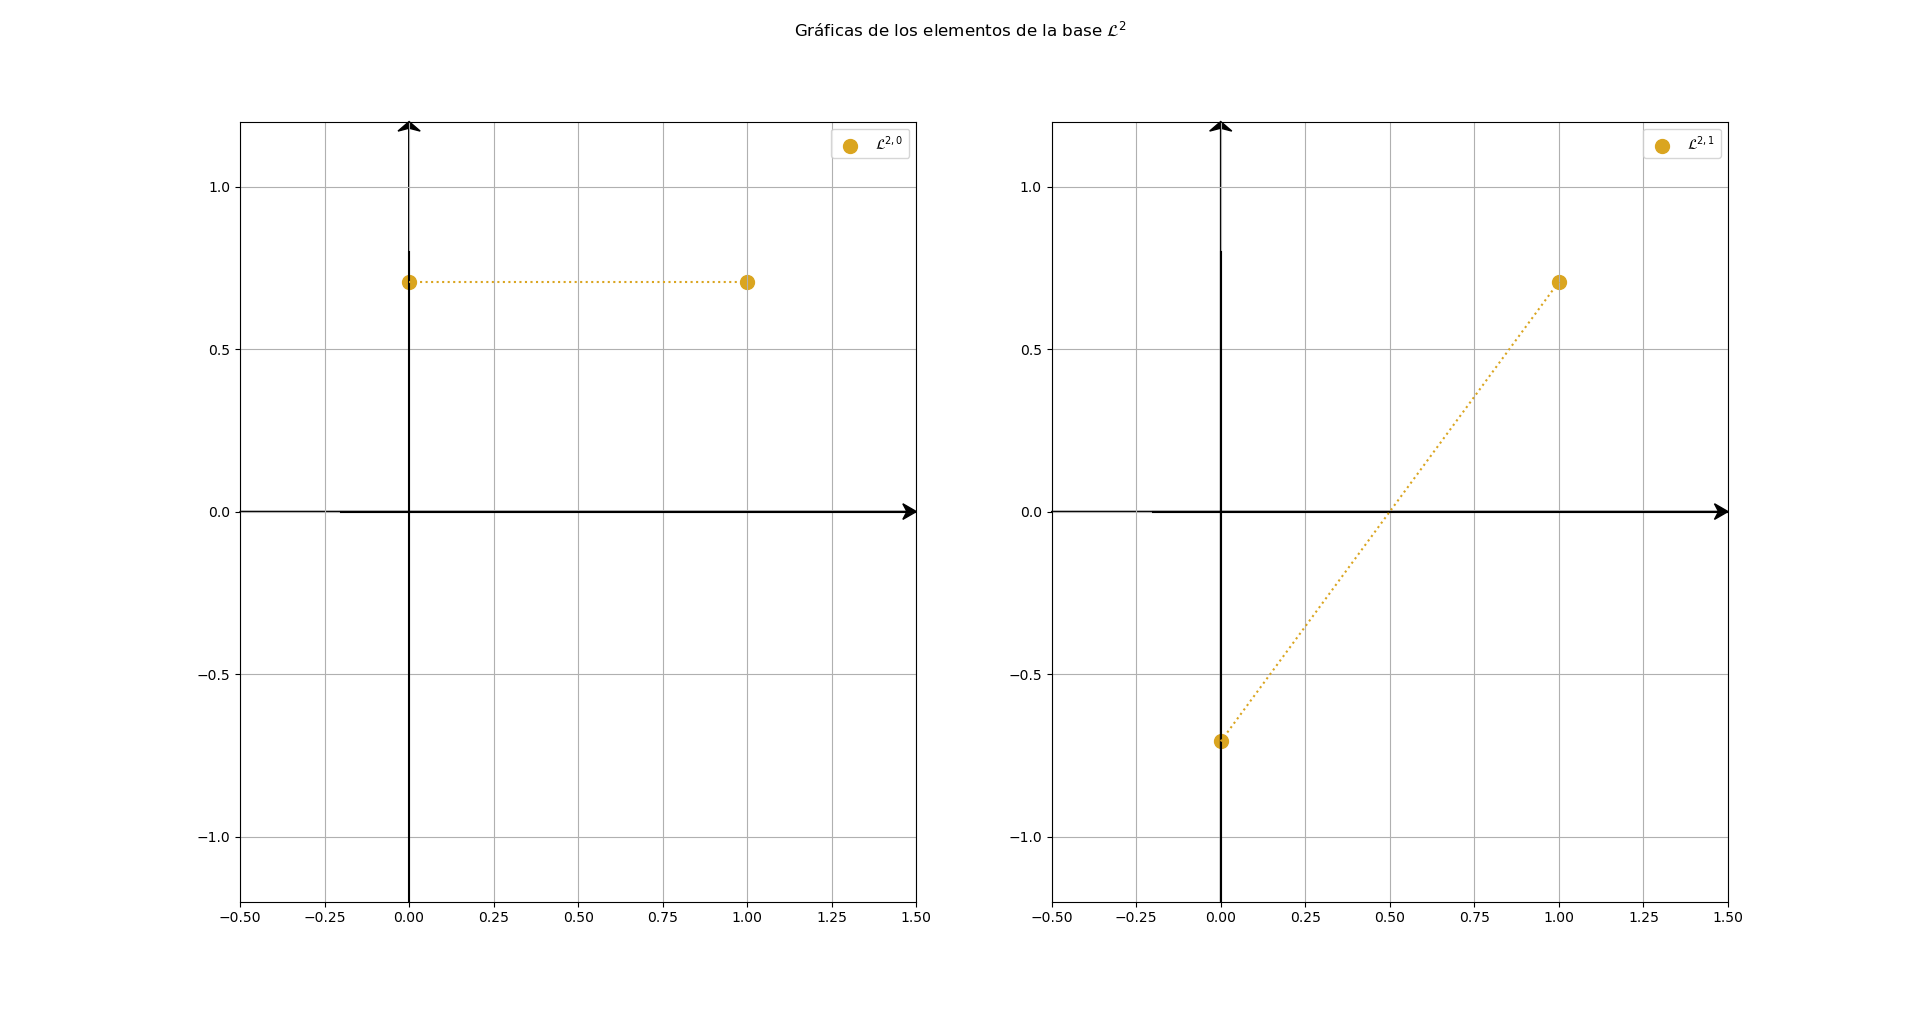
\includegraphics[scale=0.3]{graf_L2}
\end{figure}


\begin{figure}[H]
	\centering
	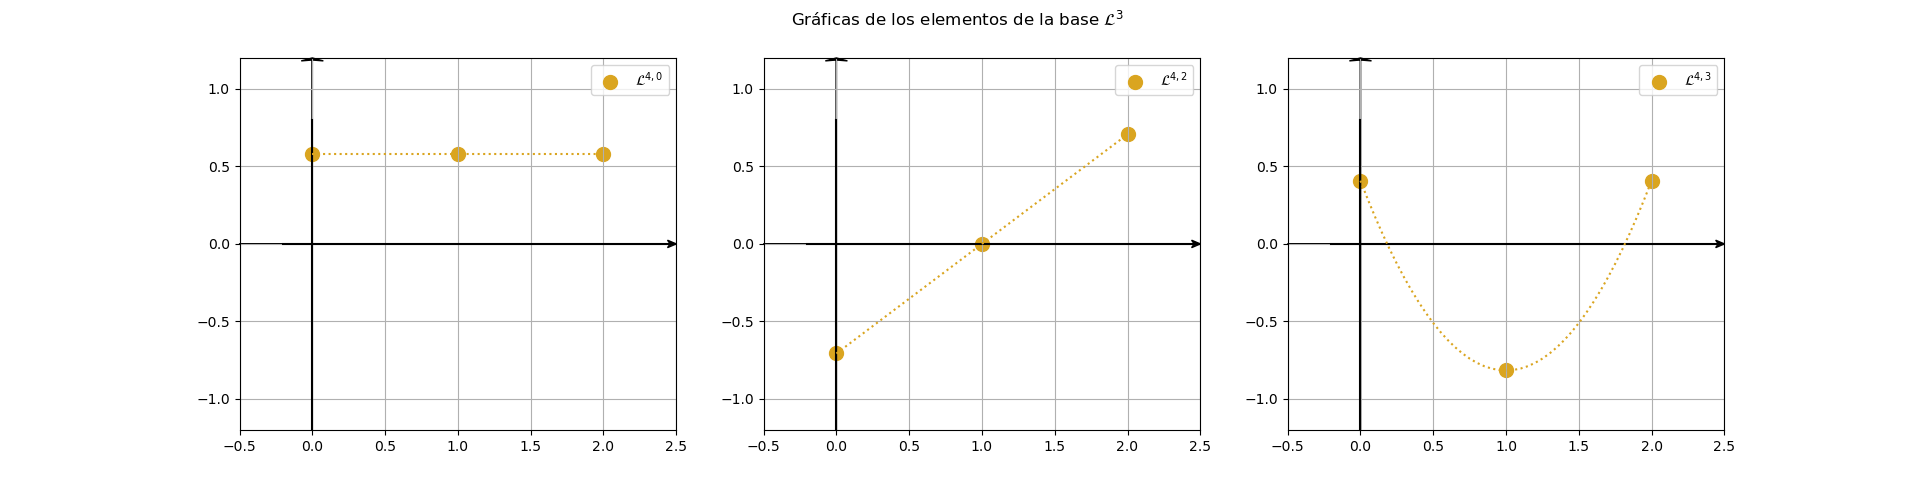
\includegraphics[scale=0.3]{graf_L3}
\end{figure}


\begin{figure}[H]
	\centering
	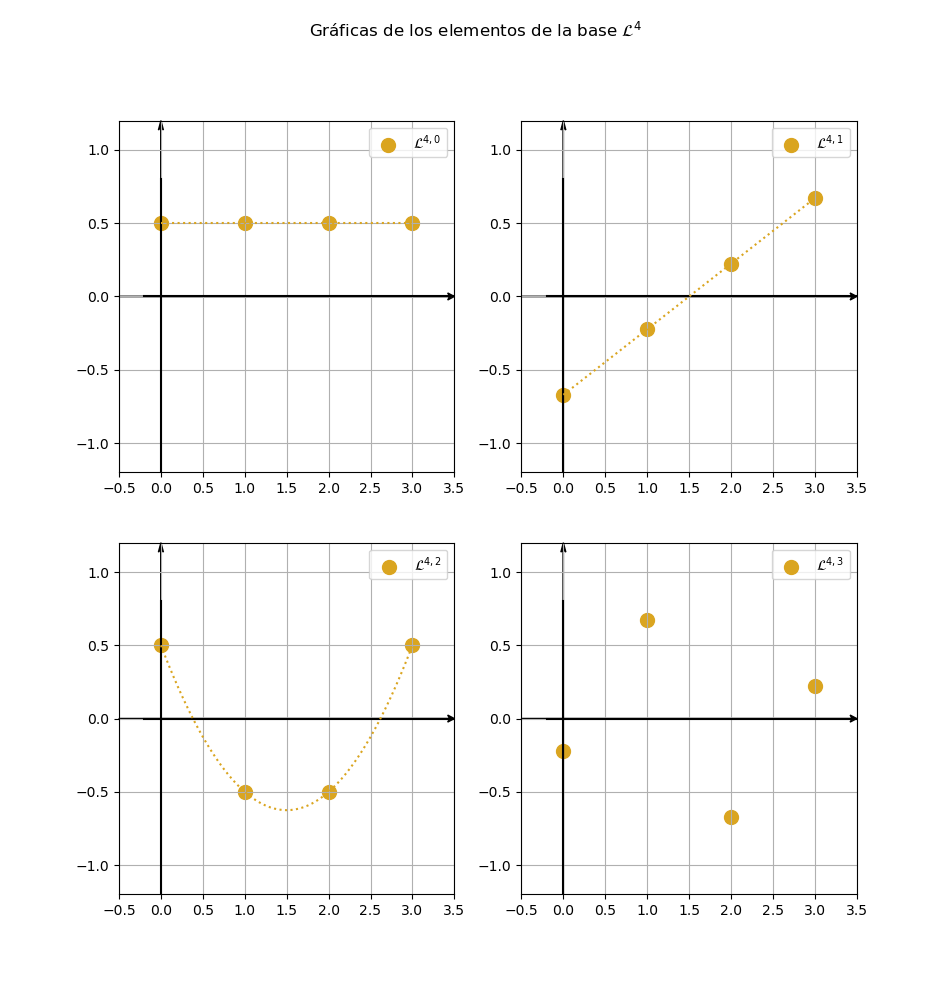
\includegraphics[scale=0.6]{graf_L4}
\end{figure}

\begin{figure}[H]
	\centering
	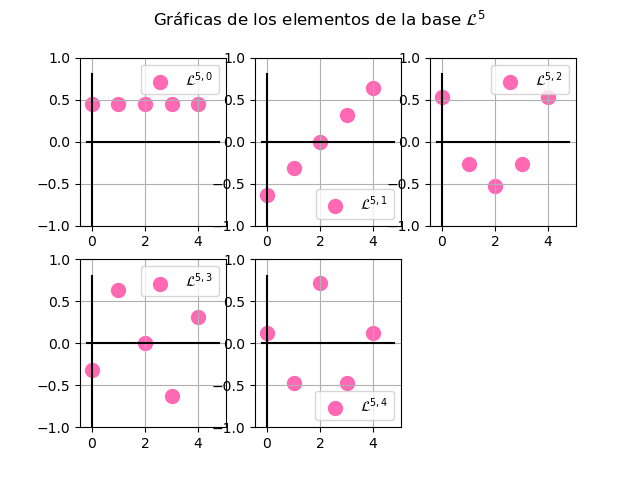
\includegraphics[scale=0.8]{graficasLegendre_5}
\end{figure}

\begin{figure}[H]
	\centering
	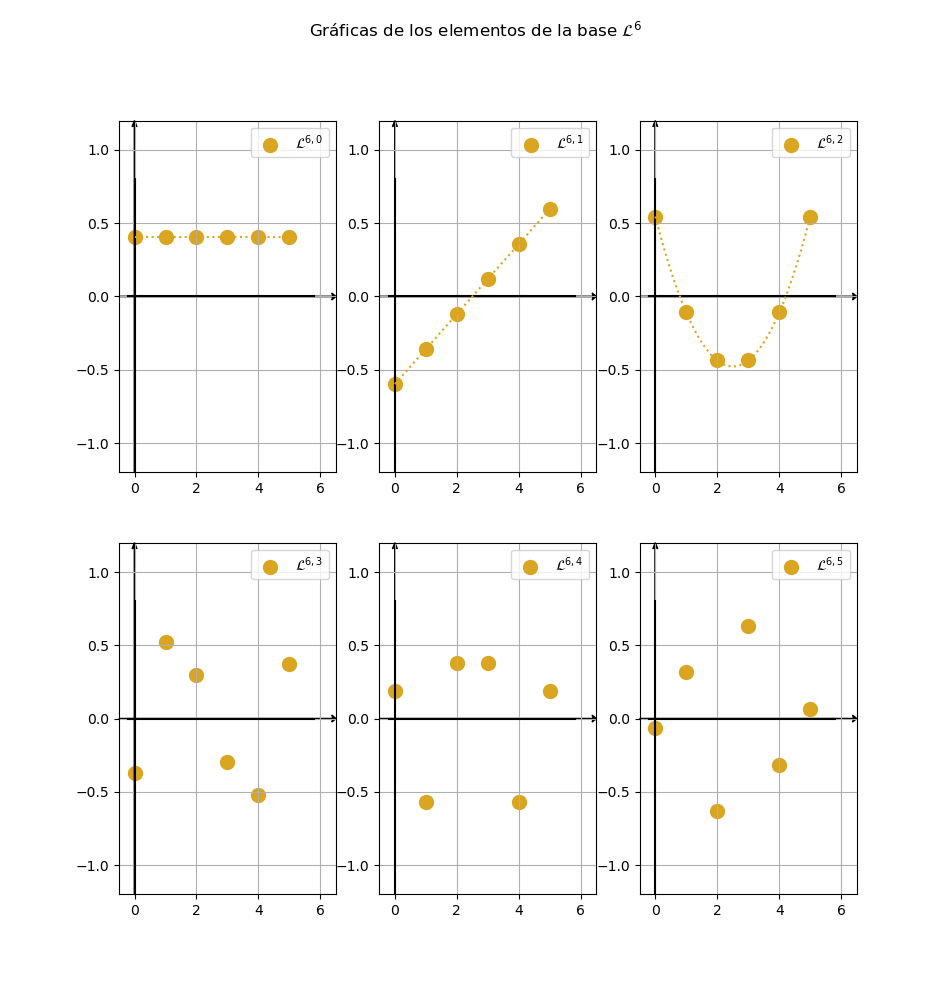
\includegraphics[scale=0.6]{graf_L6}
\end{figure}

\TODO{Deberías tambien poner
las gráficas de los vectores de orden uno, dos y tres
para dimensiones más altas. Recuerda que tienes
fórmulas simplificadas para estos.}